\documentclass{article}

\usepackage[spanish]{babel}

\usepackage[letterpaper,top=2cm,bottom=2cm,left=3cm,right=3cm,marginparwidth=1.75cm]{geometry}

\usepackage{amsmath}
\usepackage{graphicx}
\usepackage{float} 
\usepackage{pdfpages}
\usepackage[utf8]{inputenc}
\usepackage{biblatex}  
\addbibresource{sample.bib}
\usepackage[colorlinks=true, allcolors=blue]{hyperref}

\title{Reporte Pruebas Piezopulse en Schussler S.A. 24/05}
\author{Vicente Montesinos}
\DeclareUnicodeCharacter{2212}{-}
\begin{document}
\maketitle
\tableofcontents
\newpage
\section{Contextualización}

\textbf{Piezopulse} es un proyecto innovador que busca \textbf{aprovechar las vibraciones mecánicas generadas por maquinaria industrial y transformarlas en energía eléctrica almacenable}. Mediante tecnología de piezoelectricidad, estas vibraciones se convierten en electricidad, la cual se almacena en baterías para su posterior uso. De esta manera, las empresas pueden optimizar su consumo energético, reducir costos y promover prácticas más sostenibles al reutilizar energía que normalmente se perdería.\\
Actualmente, se encuentra en la \textbf{fase de evaluación de sistemas de captación}, con el objetivo de maximizar la eficiencia de conversión y minimizar las pérdidas.\\ 
Como parte de esta fase, se realizaron pruebas en \textbf{Schussler S.A.}, enfocadas en un equipo de su operación: una \textbf{impresora flexográfica}, específicamente en la sección de ventiladores. Se seleccionó esta máquina debido que es la que está \textbf{constantemente en funcionamiento sin interrupciones}. Para caracterizar el comportamiento mecánico del sistema, se midieron las vibraciones de la máquina utilizando un \textbf{acelerómetro}, lo que permitió cuantificar la amplitud y frecuencia de las oscilaciones. En paralelo, se registró el \textbf{voltaje generado por los elementos piezoeléctricos} bajo estas condiciones operativas, estableciendo una relación directa entre el movimiento mecánico y la energía eléctrica recuperable.\\
\begin{figure}[H]
    \centering
    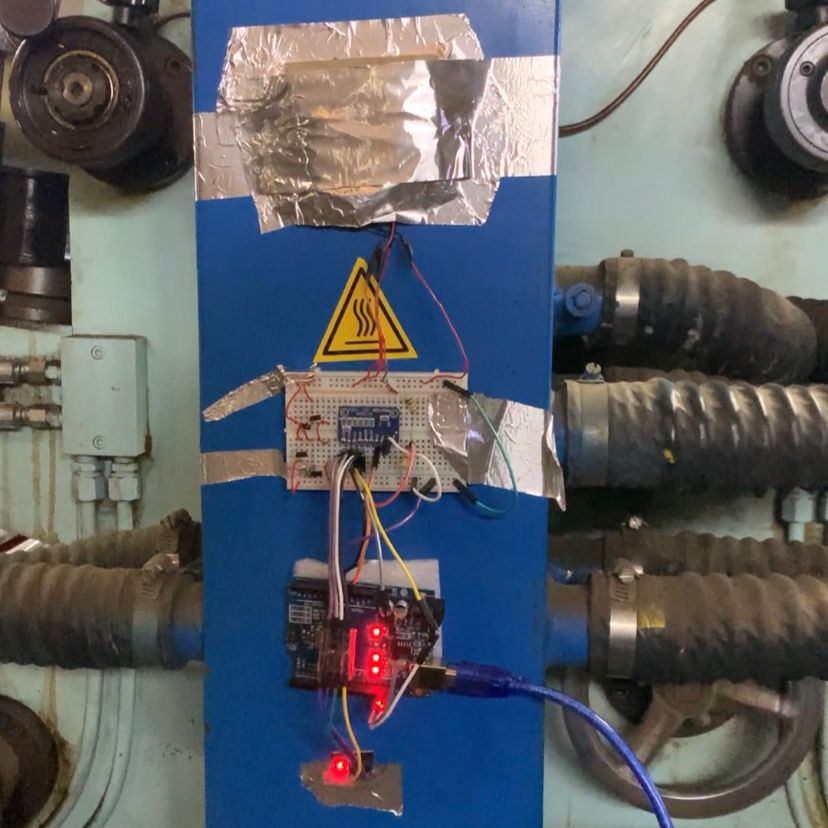
\includegraphics[width=.8\textwidth]{Sistema.jpg}
    \caption{Sistema puesto en terreno}
    \label{fig:my_label}
\end{figure}
\newpage
\section{Configuración Experimental}
El prototipo desarrollado para las pruebas en Schussler S.A. incorporó los siguientes componentes clave, configurados de la siguiente manera:
\subsection{Captación de Energía}
\begin{figure}[H]
    \centering
    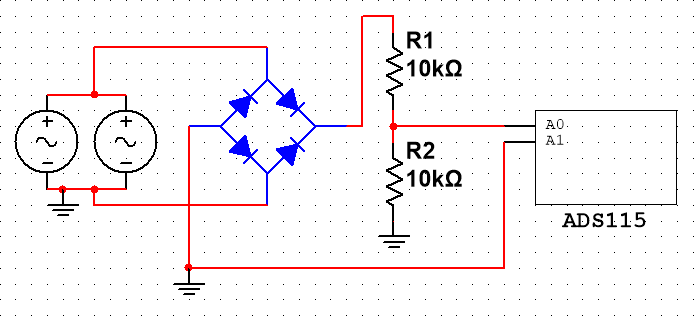
\includegraphics[scale=0.45]{ConversionAC.png}
    \caption{Esquema del sistema piezoeléctrico \textit{(Representados con una fuente alterna)}}
    \label{fig:my_label}
\end{figure}
El sistema de captación de energía consiste en \textbf{dos elementos piezoeléctricos de 35mm conectados en paralelo}, una disposición que permite maximizar la corriente de salida en respuesta a las vibraciones mecánicas. La señal alterna generada por los piezos se convierte a corriente continua mediante un \textbf{puente rectificador Schottky}, seleccionado específicamente para minimizar las pérdidas por caída de voltaje en el proceso de rectificación. Para garantizar la seguridad del sistema de medición, se implementó un \textbf{divisor resistivo de 10k$\Omega$} que asegura que el voltaje no exceda los 5V, límite máximo de entrada del conversor analógico-digital ADS1115, protegiendo así el circuito de adquisición de datos contra posibles picos de voltaje.
\begin{align*}
\text{Con diodos estándar (1N4007):} &\quad V_F \approx 0.7V \Rightarrow V_{\text{pérdida}} = 1.4V \\
\text{Con Schottky (1N5817):} &\quad V_F \approx 0.3V \Rightarrow V_{\text{pérdida}} = 0.6V \\
\end{align*}
Donde $V_F$ es la caída de voltaje directo en cada diodo.\\
\newpage
Para la correcta integración de la captación de energía, se desarrolló un \textbf{modelo 3D} para alojar los dos piezoeléctricos. Este diseño comprende dos capas de material: una primera capa de 0.5 mm de espesor diseñada para estar en contacto directo con la máquina, facilitando la transferencia de vibraciones. Superpuesta a esta, se encuentra una segunda capa de 1 mm de espesor. En el interior de estas capas, se incorporó un hueco de 1 mm de profundidad diseñado con precisión para permitir la ubicación óptima de los piezoeléctricos de 35 mm de diámetro, asegurando su estabilidad y el correcto acoplamiento mecánico para una eficiente recolección de energía.
\begin{figure}[H]
    \centering
    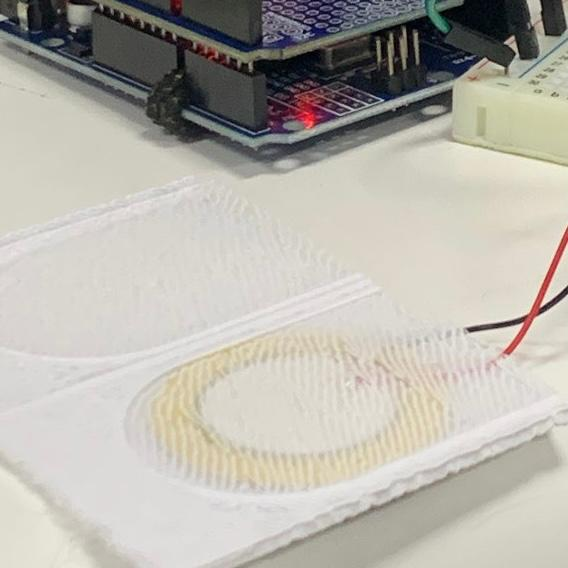
\includegraphics[scale=0.45]{3Dmodel.jpg}
    \caption{Modelo con piezoeléctrico}
    \label{fig:my_label}
\end{figure}
\subsection{Medición y Adquisición de Datos}
El sistema incorpora un acelerómetro \textbf{MPU6050} que registra con precisión las vibraciones de la impresora flexográfica a lo largo de los tres ejes espaciales (X, Y y Z). Complementando este subsensor, se emplea un \textbf{convertidor analógico-digital ADS1115} configurado en \textbf{modo diferencial}, donde la entrada positiva (A0) recibe la señal de los piezos rectificados y la entrada negativa (A1) se conecta a tierra como referencia, ofreciendo una lectura precisa del voltaje rectificado proveniente de los elementos piezoeléctricos con una resolución de 16 bits para las mediciones eléctricas. Esta configuración diferencial permite eliminar el ruido común y mejorar la precisión de las mediciones en el entorno industrial. Un \textbf{microcontrolador Arduino Uno} centraliza el procesamiento, recibiendo y almacenando los datos provenientes tanto del MPU6050 como del ADS1115.
\newpage
\subsection{Procesamiento y Almacenamiento}
El subsistema de procesamiento y almacenamiento, implementado mediante un código Arduino\cite{1}, opera en tiempo real registrando simultáneamente los datos de vibración captados por el acelerómetro MPU6050 y las mediciones de voltaje obtenidas del circuito piezoeléctrico a través del ADC ADS1115.
\begin{figure}[H]
    \centering
    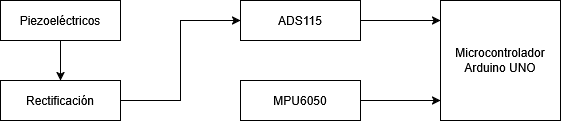
\includegraphics[scale=0.555]{SistemaGeneral.png}
    \caption{Sistema General}
    \label{fig:my_label}
\end{figure}

\section{Resultados y Análisis}

\subsection{Caracterización de la Vibración}
\subsubsection{Estadística generales por eje}
El acelerómetro tri-axial (MPU6050) instalado en la impresora flexográfica proporcionó información en las componentes \textit{AccelX}, \textit{AccelY} y \textit{AccelZ}, en unidades de ${m}/{s^2}$:
\begin{table}[H]
\centering
\begin{tabular}{lllll}
       & Mínimo & Máximo & Media & Desviación Estándar \\
AccelX & -10.52 & -8.18  & -9.36 & 0.325               \\
AccelY & -2.38  & 3.77   & 0.642 & 0.187               \\
AccelZ & -3.03  & 0.280  & -1.41 & 0.385              
\end{tabular}
\end{table}
\begin{itemize}
    \item \textbf{Eje X (AccelX):} La media cercana a -9.8 ${m}/{s^2}$ indica que este eje está alineado con la dirección de la gravedad. La desviación estándar baja (0.32 ${m}/{s^2}$) sugiere que las vibraciones en este eje son mínimas o casi inexistentes. La máquina permanece estable en este eje.
    \item \textbf{Eje Y (AccelY):} La aceleración promedio es de 0.64 ${m}/{s^2}$, con una desviación moderada (0.19 ${m}/{s^2}$), lo que indica presencia de vibración ligera. El rango desde -2.38 a 3.77 ${m}/{s^2}$ muestra que existen picos en ambos sentidos, lo que sugiere oscilaciones transversales posiblemente inducidas por el funcionamiento de la máquina.
    \item \textbf{Eje Z (AccelZ):} Este eje muestra una aceleración promedio negativa (-1.41 ${m}/{s^2}$) con la mayor desviación estándar de los tres (0.38 ${m}/{s^2}$), y un rango significativo (-3.03 a 0.28 ${m}/{s^2}$). Esto indica que el eje Z es el más afectado por las vibraciones de la máquina, probablemente en la dirección vertical u otra perpendicular al plano principal del equipo.
\end{itemize}
En resumen, el eje más vibrante es el Z, seguido del Y, mientras que el X está dominado por la gravedad (poca vibración útil).
\subsubsection{Análisis Espectral (FFT)}
\begin{figure}[H]
    \centering
    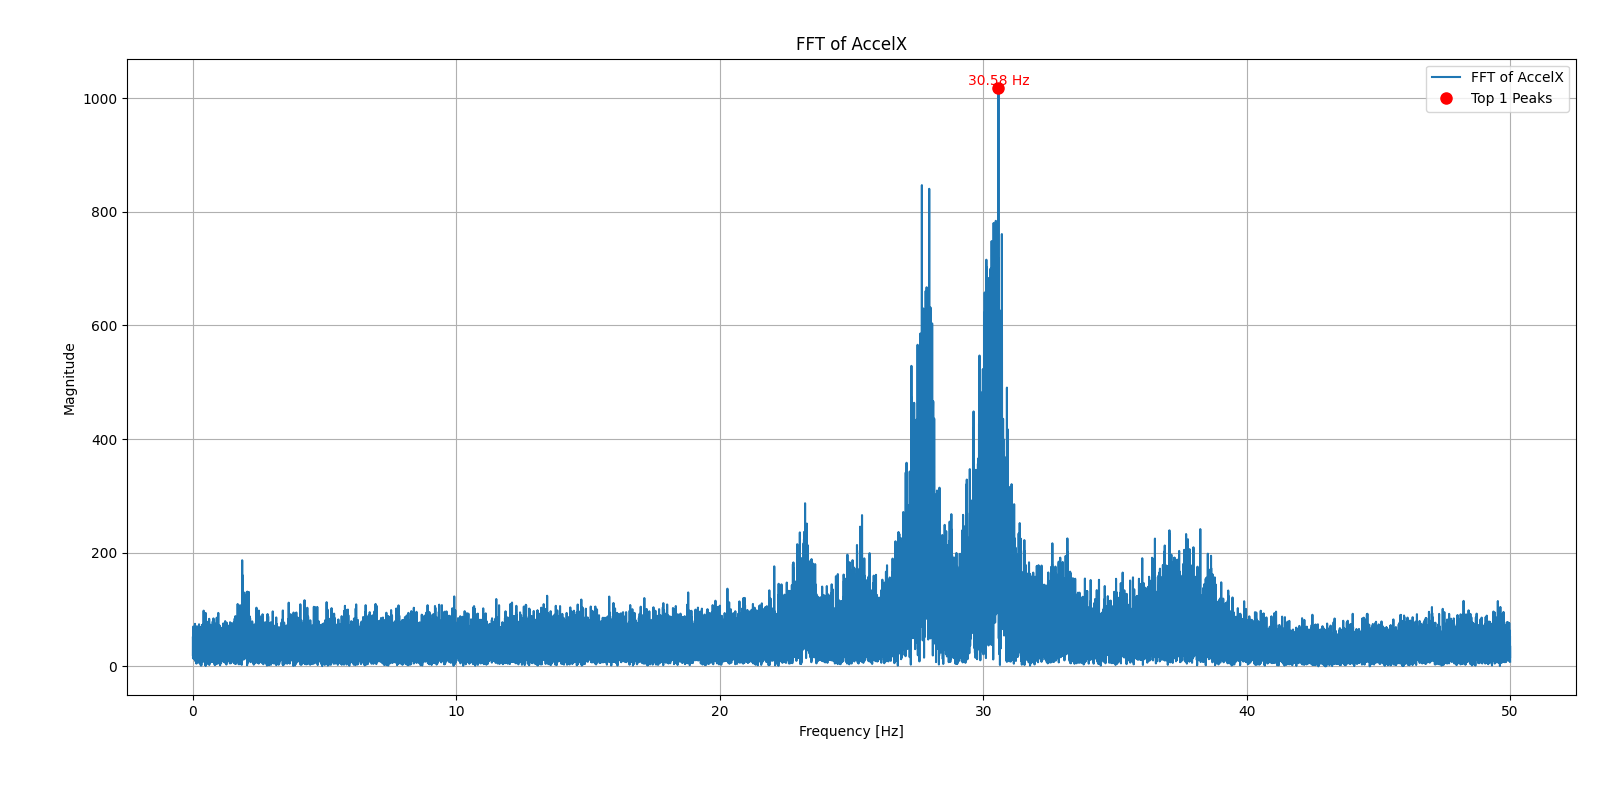
\includegraphics[width=\textwidth]{fftx.png}
    \caption{Análisis espectral de la aceleración en el eje X}
    \label{fig:my_label}
\end{figure}
\begin{figure}[H]
    \centering
    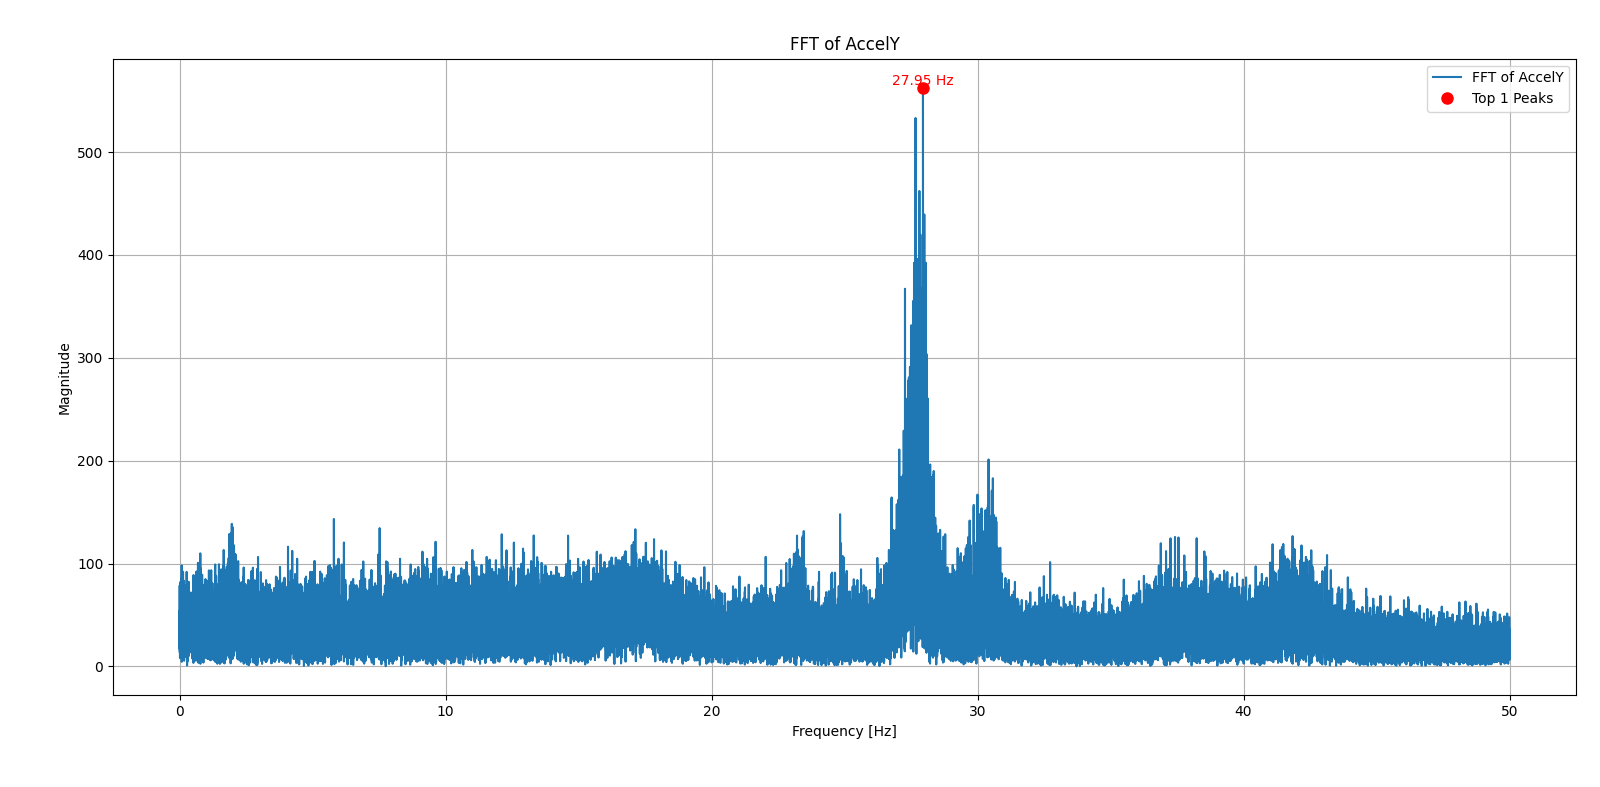
\includegraphics[width=\textwidth]{ffty.png}
    \caption{Análisis espectral de la aceleración en el eje Y}
    \label{fig:my_label}
\end{figure}
\begin{figure}[H]
    \centering
    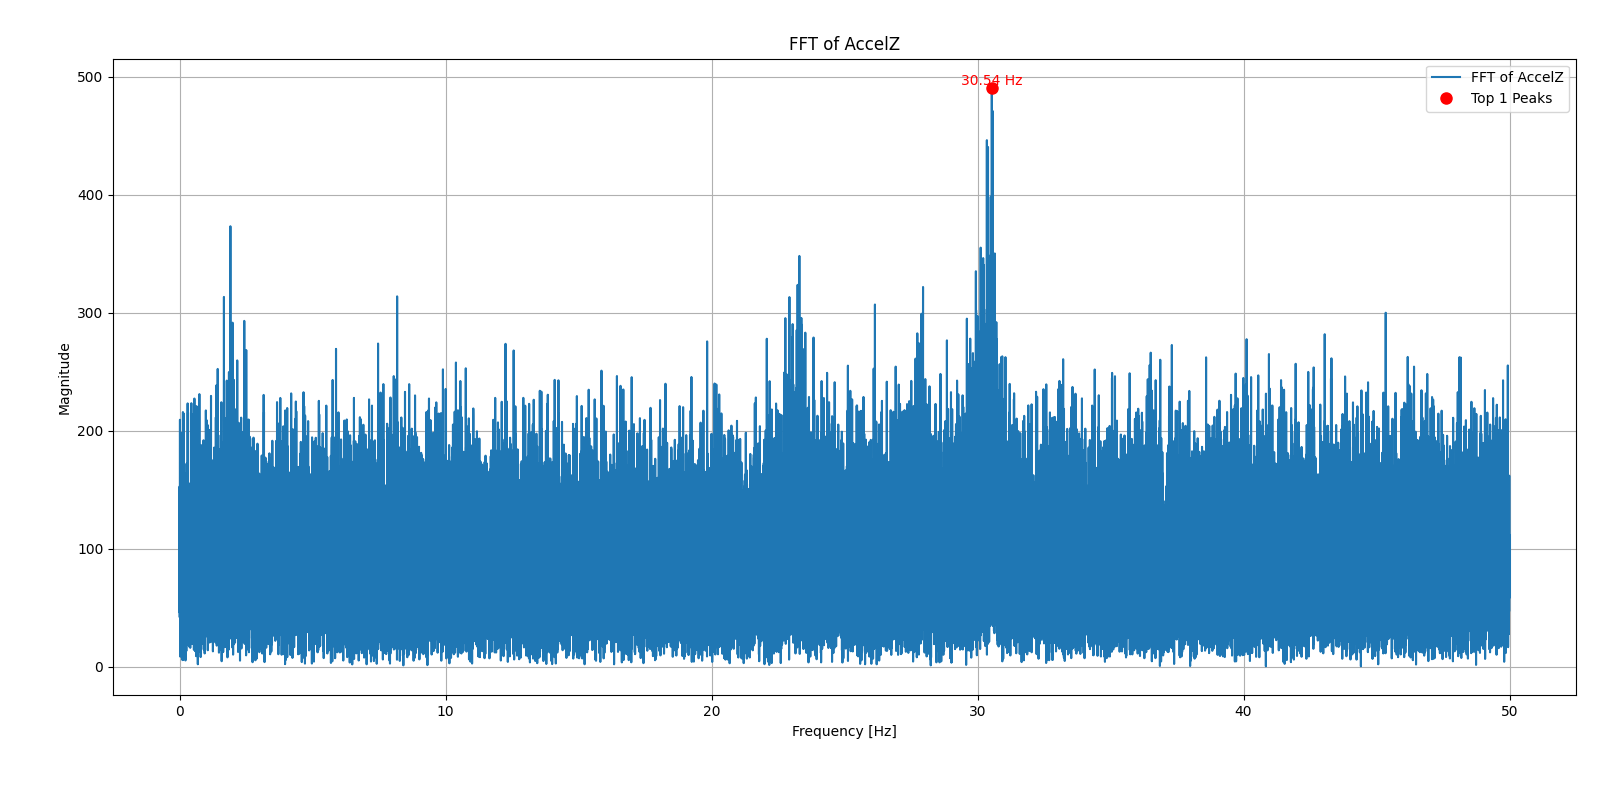
\includegraphics[width=\textwidth]{fftz.png}
    \caption{Análisis espectral de la aceleración en el eje Z}
    \label{fig:my_label}
\end{figure}
Se aplicó una transformada rápida de Fourier (FFT) a las señales de aceleración en los tres ejes (AccelX, AccelY, AccelZ) para identificar las componentes de frecuencia presentes durante el funcionamiento de la impresora flexográfica. Se observó un pico dominante de amplitud en torno a los \textbf{30 Hz en los tres ejes}.
Esta frecuencia es relevante para el proyecto, ya que si el sistema piezoeléctrico tiene una frecuencia de resonancia cercana a 30 Hz, se maximiza la eficiencia de conversión energética.
\subsection{Energía piezoeléctrica}
Durante la operación de la máquina, se registró el voltaje generado por un conjunto de piezoeléctricos conectados en paralelo, acoplados mecánicamente a su estructura. La señal fue rectificada y atenuada mediante una divisora resistiva (2 resistencias de 10k$\Omega$) antes de ser medida por un conversor ADS1115 en modo diferencial.
\begin{table}[H]
\centering
\begin{tabular}{lllll}
       & Mínimo & Máximo & Media & Desviación Estándar \\
Voltaje & 0.00 & 10.10  & 0.664 & 0.653               
\end{tabular}
\caption{Estadísticas del voltaje producido por los piezoeléctricos (en milivolts)}
\end{table}
Aunque los niveles de voltaje son bajos, se confirma que los piezoeléctricos \textbf{generan señal eléctrica a partir de las vibraciones reales de la máquina}. La aparición de voltajes máximos cercanos a 10mV demuestra que en ciertas condiciones, posiblemente a picos de vibración, el sistema puede captar energía de forma significativa.
La media baja indica que el sistema no opera continuamente en esas condiciones óptimas, lo que es esperable dado que el acoplamiento no está sintonizado aún para 30 Hz.\\
En conclusión, el sistema es \textbf{capaz de convertir vibraciones mecánicas reales en energía eléctrica, incluso en condiciones no óptimas} y la señal generada puede ser utilizada como \textbf{fuente de energía si se incorpora un sistema de acumulación} y regulación.
\newpage
\subsection{Relación entre vibración y generación}
Ya que se observó que el eje más vibrante es el Z, haremos la comparación entre el voltaje generado por los piezoeléctricos y la vibración en el eje Z.
\begin{figure}[H]
    \centering
    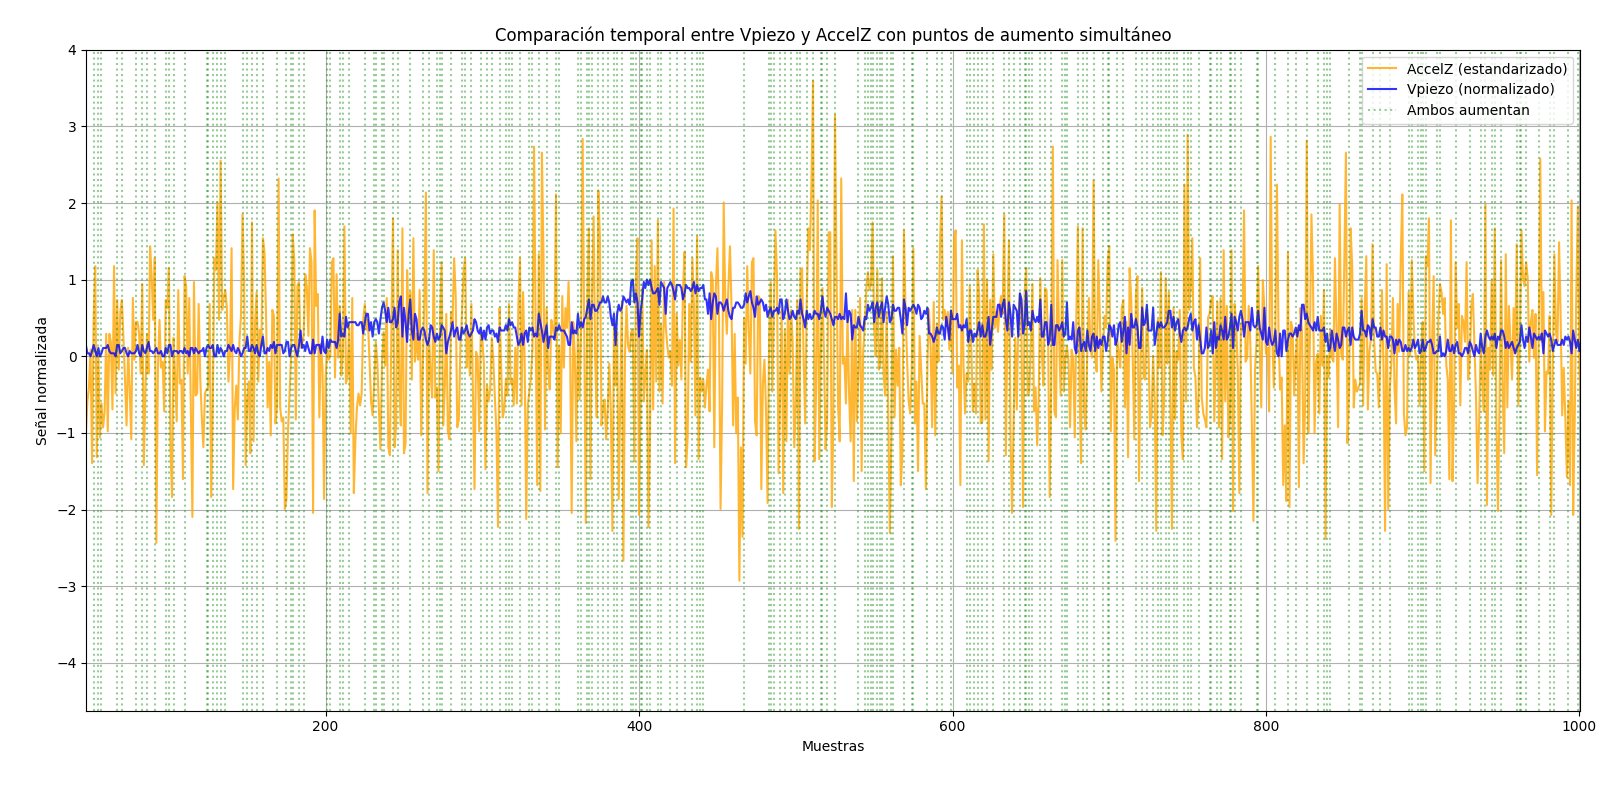
\includegraphics[width=\textwidth]{AccelZxVpiezo.png}
    \caption{Extracto de las muestras obtenidas.}
    \label{fig:my_label}
\end{figure}
Se encontraron 13331 puntos donde ambos valores aumentan al mismo tiempo, estos puntos se muestran reflejados en verde en el gráfico.
Se evidencian coincidencias temporales entre los picos de aceleración y los aumentos de voltaje. Esto confirma que el sistema piezoeléctrico responde de forma efectiva a la vibración mecánica, transformando parte de la energía cinética en voltaje utilizable.

\section{Conclusión y próximos pasos}
La prueba realizada sobre una impresora flexográfica permitió validar el concepto fundamental del sistema PiezoPulse: \textbf{convertir vibraciones mecánicas reales en energía eléctrica utilizable} mediante piezoeléctricos. Los principales hallazgos son:
\begin{itemize}
    \item Se observó una frecuencia dominante de \textbf{vibración en 30 Hz}, presente en los tres ejes del acelerómetro, lo que indica una oscilación estructural importante en la máquina.
    \item El eje Z mostró la mayor variabilidad, coincidiendo con la mayor actividad vibracional y con los momentos de mayor voltaje generado por los piezoeléctricos.
    \item El voltaje piezoeléctrico alcanzó \textbf{valores de hasta 10.1mV, con una media de 0.66mV}, demostrando la capacidad del sistema para captar energía real desde el entorno.
\end{itemize}
En conjunto, los resultados respaldan la viabilidad del enfoque PiezoPulse y permiten avanzar hacia una implementación práctica.
\\
Para escalar y mejorar el sistema, se proponen las siguientes acciones:
\begin{itemize}
    \item Probar con diferentes conexiones de piezoeléctricos (paralelo o serie) y escalar el número de piezoeléctricos ocupados
    \item Utilizar piezoeléctricos con una frecuencia de resonancia más cercana a los 30 Hz observados o evaluar otras estructuras mecánicas resonantes.
    \item Integrar un sistema con diodos Schottky + supercondensador o batería Li-ion para acumular la energía generada.

\end{itemize}
\newpage
\begin{thebibliography}{1}

\bibitem{pp}
A.~M.~Z. Vicente, ``Piezopulse Data,'' \emph{GitHub repository}, 2025. [Online]. Available: \url{https://github.com/mzvic/Piezopulse}. Commit: 139a056b413fea6309fc6aff419420ad5c2312db

\end{thebibliography}
\printbibliography

\end{document}
